\chapter{Contextualització}

\label{Contextualitzacio}

\section{Presentació i justificació de la temàtica}

En les darreres dècades els sistemes software han evolucionat fins al punt d’esdevenir elements clau i imprescindibles de les activitats primàries de qualsevol empresa, organització o institució. La gestió de la informació, els protocols i controls de seguretat, els processos de negoci, etc., són els reptes als quals els CIO de moltes empreses s’han d’enfrontar. Aquests reptes i els seus resultats depenen, en gran mesura, del comportament dels sistemes software que entren en joc dins aquestes activitats. Adicionalment, la quantitat de productes software exposats com a serveis o aplicacions mòbils ha incrementat dràsticament. Fet que deriva en el sorgiment d'una gran varietat de contexts i entorns d'execució entre els grans volums d'usuaris que aquests sistemes poden tenir. \\

És per aquest motiu que eventualment ha anat prenent força un concepte basat en l’estudi i control de qualitat dels sistemes software: el monitoratge. Com a part de la vida professional d’un enginyer de software, la supervisió i control dels components i sistemes amb els què treballa és un concepte clau amb el qual, d’una forma o altra, ha d’estar familiaritzat. Però el problema que plantegem aquí va més enllà: després del repte de monitorar els sistemes, ens hem de plantejar com dissenyar, gestionar i adaptar aquest monitoratge.\\

Els reptes que aquestes tasques plantegen i que aquest projecte treballa són diversos. Entre d'altres, cal valorar el disseny i les característiques tècniques dels monitors, la seva configuració i la capacitat d'adaptabilitat. En relació amb aquest últim aspecte, també cal valorar com s'emmagatzemen i es gestionen els detalls relacionats amb la configuració dels monitors, i establir interaccions de la manera més genèrica possible per facilitar l'extensibilitat.\\

Tal i com veurem més endavant a l’apartat \textit{2.3. Estat de l’art}, existeix una àmplia recerca que actualment treballa i desenvolupa projectes en relació a aquest àmbit. El potencial d’estudi que ofereix resulta d’un alt interès a causa de la possibilitat de recerca i síntesi i als diferents aspectes i criteris sobre els quals es pot treballar.\\

Així, tant com estudiant com a futur professional del sector de l’enginyeria del software, es poden contemplar diversos criteris per treballar en aquesta temàtica:
\begin{itemize}
\item Un aprofundiment en els coneixements de l’enginyeria i els sistemes software
\item Treball i recerca en conceptes de control de qualitat, fiabilitat i millora de l'experiència de l'usuari
\item Possibilitat de col·laborar i aprofundir en un tema de recerca d’actualitat dins l’enginyeria de serveis i els sistemes d’informació
\item Plantejament d’un projecte complet que pugui servir a tercers interessats en l’estudi de sistemes de monitoratge autoadaptatius
\end{itemize}  

\subsection{Identificació dels stakeholders}

Les diferents fases que engloben aquest projecte deriven en l'obtenció d'un producte final, orientat a la seva aplicació pràctica. Com a tal, els documents generats i els components dissenyats i implementats esdevenen productes propis dins el context del monitoratge de sistemes software. Com a tals, aspectes que s'exposaran al llarg d'aquest document (el disseny i implementació d'una arquitectura genèrica pels monitors, la gestió de les configuracions, etc.) poden resultar d'utilitat per a agents externs a la pròpia autoria del projecte.\\

Podem considerar, per tant, que podrà ser una eina d’interès pels principals stakeholders, que vindrien a ser:
\begin{itemize}
\item \textbf{Desenvolupadors i enginyers software}. Aquells agents al càrrec del control de qualitat de sistemes softwares de diverses naturaleses. Els conceptes treballats, el plantejament de problemàtiques, i el producte generat, poden aportar valor de qualitat al sector treballant, per una banda, en la síntesi i recopilació de la informació actual, i per altra banda, aportant propostes i solucions pròpies basades en l’experiència del desenvolupament del projecte.
\item \textbf{Gestors de projecte i experts en Sistemes d'Informació}. La gestió de la informació, el tractament i el seu potencial poden resultar afectats gràcies a la capacitat de recol·lecció de dades del sistema de monitoratge, així com els criteris de revisió i control de qualitat, que permeten analitzar i obtenir informació fiable.
\item \textbf{Usuaris finals dels sistemes monitorats}. De forma indirecta, es veuran afectats degut a les conseqüències del monitoratge dut a terme per aquest sistema de monitoratge o d’altres derivats dels conceptes treballats al llarg d’aquest projecte.
\end{itemize}

%----------------------------------------------------------------------------------------
%	SECTION 2
%----------------------------------------------------------------------------------------

\section{Estat de l'art}

Per tal de plantejar les necessitats i projeccions del treball, així com les vies de desenvolupament del projecte, és necessari conèixer quina és la situació del monitoratge autoadaptatiu de sistemes software en la recerca actual.\\

En primer lloc, cal conéixer l’entorn referent als sistemes software autoadaptatius: és a dir, aquells que seran l’objectiu de monitoratge del nostre sistema de monitoratge (que no deixa de ser un altre sistema software autoadaptatiu). És interessant veure com la recerca i la investigació planteja, de forma pràcticament correlacionada, els conceptes de sistema autoadaptatiu i monitoratge.\\

\begin{figure}
\centering
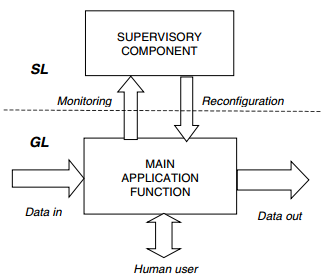
\includegraphics[width=8cm]{Figures/Figure1}
\decoRule
\caption[Arquitectura de sistemes auotadaptables monitorats]{Arquitectura de sistemes autoadaptables monitorats}
\label{fig:Figura1}
\end{figure}

De fet, documents de caràcter acadèmic tals com \textit{“An Approach to Self-adaptive Software Based on Supervisory Control”} , publicat per la Vanderbilt University de Nashville (USA), plantegen una arquitectura d’autoadaptabilitat per sistemes software basada en la supervisió o monitoratge. Tal com podem veure a la Figura 2.1, destaquem dos components principals: l’aplicació principal, o \textbf{Main Application Function}, equivalent al sistema software (servei web, aplicació mòbil, etc.) encarregat d'una funcionalitat específica i sobre el qual volem realitzar el control de qualitat; i el component supervisor, o \textbf{Supervisory Component}, que s'encarrega d'executar aquest control de qualitat.\\

La interacció i arquitectura plantejada en la figura és relativament senzilla. El component software a avaluar forma part del domini del sistema a avaluar (\textit{ground-level}, GL). En la seva activitat, aquesta aplicació o sistema rep una sèrie de dades (que dependrà de la naturalesa i objectiu del sistema), i produeix uns resultats en base a aquest \textit{input}. Paral·lelament, com qualsevol sistema orientat a l'ús, existeix una interacció sistema-usuari. Més enllà del domini i les característiques pròpies dels sistemes software, es presenta l'entorn corresponent al sistema de supervisió o monitoratge (\textit{supervisory-level}, SL). En aquest nivell trobem des d'un punt de vista lògic el component de supervisió o monitor, que interacciona amb l'aplicació principal de dues formes diferents:

\begin{itemize}
\item \textbf{Monitoratge}. Procés d'interacció entre el component principal i el monitor on el primer envia informació al segon. L'aplicatiu produeix, com a conseqüència de la seva activitat, informació i dades que envia com a \textit{output} al monitor. Aquesta informació ha d'estar prèviament definida i estructurada, de tal manera que el monitor sigui capaç d'interpretar-la.
\item \textbf{Reconfiguració}. El monitor procesa les dades que rep com a input del monitoratge i, segons els criteris d'adaptabilitat establerts, aplica els canvis o reconfiguracions pertinents en el sistema software monitorat. D'aquesta manera, la lògica encarregada d'interpretar la informació i prendre decisions d'adaptabilitat (SL) queda totalment separada de la lògica del domini de l'aplicatiu (GL).
\end{itemize}

Partint d'aquest punt, aquest document estableix les premisses del monitoratge i les necessitats de reconfiguració d’aquests tercers sistemes softwares, la naturalesa dels quals és diversa i heterogènia. Noti's que, de fet, l'anterior disseny presenta una arquitectura genèrica aplicable a qualsevol entorn software, independentment de la naturalesa del domini monitorat. Tot i així, existeix una àmplia recerca especialitzada: publicacions com \textit{"Agent Based Services for Negotiation, Monitoring and Reconfiguration of Cloud Resources”} , publicada per la universitat de Nàpols (Itàlia), es centren en analitzar els requisits, necessitats i funcions principals del monitoratge i reconfiguració de sistemes i recursos al núvol (p.e. serveis web).\\

La documentació i bibliografia referent als sistemes software autoadaptables i als sistemes de supervisió i monitoratge és molt àmplia. Tot i així, si focalitzem la recerca a la problemàtica a resoldre, és a dir, l’autoadaptabilitat i reconfiguració dels sistemes de monitoratge, no trobem un treball tan profunditzat i específic com en el cas prèviament explicat.\\

En alguns documents, com per exemple el ja esmentat publicat per la University of Nashville, es mencionen criteris del disseny de la capa de supervisió, entre els quals entren en joc, p.e., factors com la previsió d’errors a la capa de l’aplicatiu principal, o ve esdeveniments/disparadors inesperats. I, com és lògic, una reacció i canvis per part del sistema de monitoratge. \\

En altres documents, tals com “Self-reconfiguration of service-based systems: a case study for service level agreements and resource optimization” , publicat per IBM, es defineixen models autònoms d’autoadaptabilitat i reconfiguració autònoma, basats en tècniques de detecció d’esdeveniments i canvis en el propi sistema. Conceptes com l’anàlisi de l’estat del sistema, el monitoratge i l’execució d’una reconfiguració entren en joc dins d’aquest pla.

%-----------------------------------
%	SUBSECTION 2
%-----------------------------------

\subsection{Projecte SUPERSEDE}

Com a part de l'estat de l'art i punt de partida pel desenvolupament del sistema, cal introduïr el projecte SUPERSEDE (https://www.supersede.eu/). Aquest projecte forma part del \textit{Horizon 2020 Programme}, un programa de recerca i innovació financiat i gestionat per la Unió Europea. Actualment, compta amb la participació de diverses empreses, fundacions i universitats, entre les quals s'inclou la pròpia UPC. \\

Aquest projecte planteja una proposta del cicle de vida i la gestió dels serveis software i les aplicacions, amb l'objectiu final similar al plantejat com a premisa d'aquest Treball de Final de Grau: millorar la qualitat de l'execució dels sistemes software i, en conseqüencia, l'experiència de l'usuari final en l'interacció amb aquests sistemes. \\

Dins aquest cicle de vida, orientat al control de qualitat dels sitemes software, es proposen 4 fases:

\begin{enumerate}
\item \textbf{Col·lecció}. L'obtenció i emmagatzematge de dades que puguin resultar d'interès pel control de qualitat. La naturalesa d'aquestes dades (així com el format i altres criteris) dependran de l'objectiu d'aquest anàlisi i el tipus de dades tractat. Així, aquestes poden incloure desde dades purament analítiques (p.e. \% de disponibilitat del sistema) o bé contextuals (p.e. missatges o continguts introduïts al sistema).
\item \textbf{Anàlisi}. Les dades obtingudes en la fase anterior tenen un significat, una informació que el sistema ha de ser capaç d'extreure i comprendre. En aquesta fase, les dades es transformen en coneixement en relació a l'estat del sistema, a través de diverses tècniques anal·lítiques, de nou en funció del marc d'estudi i el context. Per exemple, es podrien valorar tècniques d'anàlisi de llenguatge natural per estudiar les valoracions d'usuaris introduïdes a un sistema.
\item \textbf{Decisió}. El coneixement produït a l'anterior fase genera la capacitat de prendre decisions de millora i actuació sobre el sistema software. És a dir, deriva en una o vàries suggerencies d'adaptació. Les eines de presa de decisions entren en joc en aquesta fase, rebent com a entrada la informació i, a partir dels criteris i paràmetres definits en relació a aquesta informació, es produeix la suggerència d'adaptació del sistema.
\item \textbf{Adaptació}. Un cop el sistema ha estat capaç de produïr de forma automàtica una suggerència de millora o adaptació del sistema, aquesta s'aplica sobre el component monitoritzat amb l'objectiu de millorar l'experiència de l'usuari. Arribats a aquest punt, es tanca el cicle de control de qualitat, reflectint la transformació de l'input de la fase de col·lecció, les dades, fins a l'output d'aquesta darrera fase, l'adaptació del sistema.
\end{enumerate}

\begin{figure}
\centering
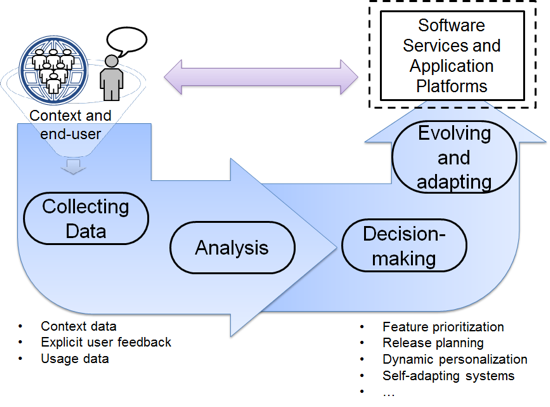
\includegraphics[width=10cm]{Figures/Figure2}
\decoRule
\caption[Cicle de vida i entorn proposat per SUPERSEDE]{Cicle de vida i entorn proposat per SUPERSEDE}
\label{fig:Figura1}
\end{figure}

La Figura 2.2 resumeix aquest cicle de vida i les característiques del context de les seves fases. Tal i com es pot observar, la principal font de dades amb les quals aquest control de qualitat es nodreix es l'experiència de l'usuari final, el context on s'executa aquesta aplicació o sistema i les dades generades del propi ús i funcionament del sistema. És, per tant, un aspecte clau l'obtenció de \textbf{dades en execució real}, que seran les que ens permetin aplicar aquest cicle regularment. Regularitat que serà crucial per satisfer l'objectiu d'anàl·lisi de la qualitat del sistema: només amb dades actuals i constants serem capaços de conéixer l'activitat real del nostre sistema i actuar en conseqüència.\\

En aquest context identifiquem per tant 4 sectors o subsistemes amb un objectiu específic que, integrats, serveixen a un propòsit genèric. Si ens plantegem com encaixa aquest model dins el nostre tema d'estudi (és a dir, l'adaptabilitat dels sistemes de monitoratge) podem establir una relació directa amb les fases de \textbf{col·lecció} de dades i \textbf{adaptació}. Dins aquesta primera fase de col·lecció, necessitem definir un sistema capaç d'obtenir aquestes dades, en funció dels sistemes a controlar i de l'interès que tinguem sobre aquests sistemes. Aquest sistema de \textbf{monitoratge} estarà composat per un conjunt definit de monitors, encarregats de recollir aquesta informació. Per altra banda, si volem dotar a aquest sistema de monitoratge d'adaptabilitat, i per tant, garantir un control de qualitat sobre aquests monitors, necessitem establir un sistema que gestioni l'activitat dels monitors i defineixi adaptacions a aplicar sobre aquests monitors.\\

Pel desenvolupament d'aquest projecte, ens centrarem en aquestes dues parts: el sistema encarregat de la fase de col·lecció de dades (monitors), i el sistema encarregat de gestionar i aplicar les adaptacions sobre aquest sistema de col·lecció. De la mateixa manera, es treballa la integració entre aquests dos components, per generar com a resultat final l'objectiu d'aquest projecte: un sistema de monitoratge autoadaptable, heterogeni i distribuït.